\documentclass{article}
\usepackage{amsfonts, amsmath, amssymb, amsthm} % Math notations imported
\usepackage{enumitem}
\usepackage{graphicx}
\usepackage{setspace}
\usepackage{indentfirst}
\usepackage[margin=1in]{geometry}
\graphicspath{{./images/}} % Path to images

% \begin{figure}[htb!]
%      \centering
%      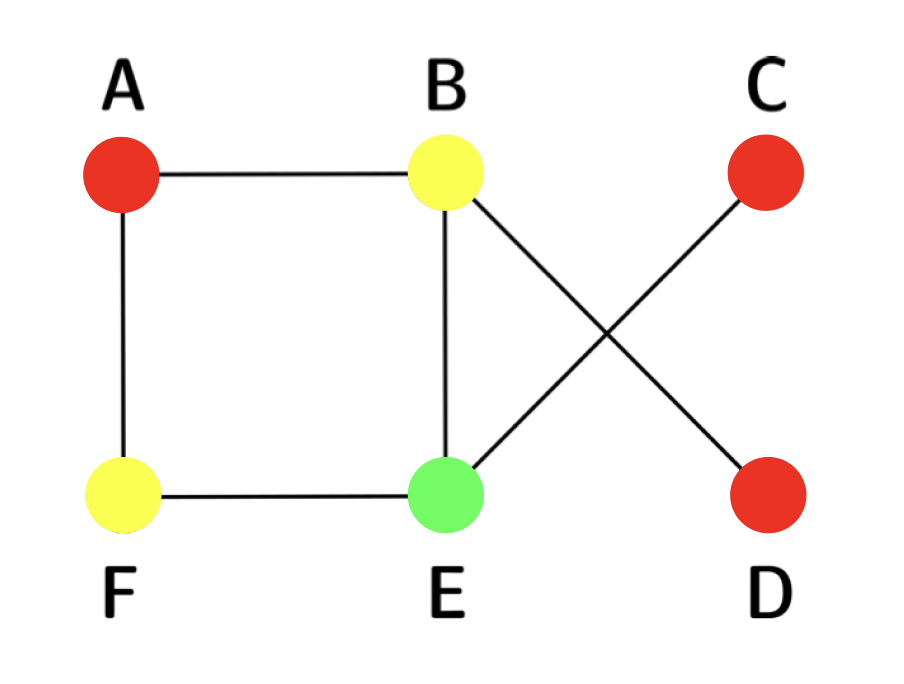
\includegraphics[scale=0.5]{coloring.png}
%      \caption{Coloring of the graph.}
% \end{figure}

% \begin{figure}[htb]
%     \qquad
%     \begin{minipage}{.4\textwidth}
%         \centering
%         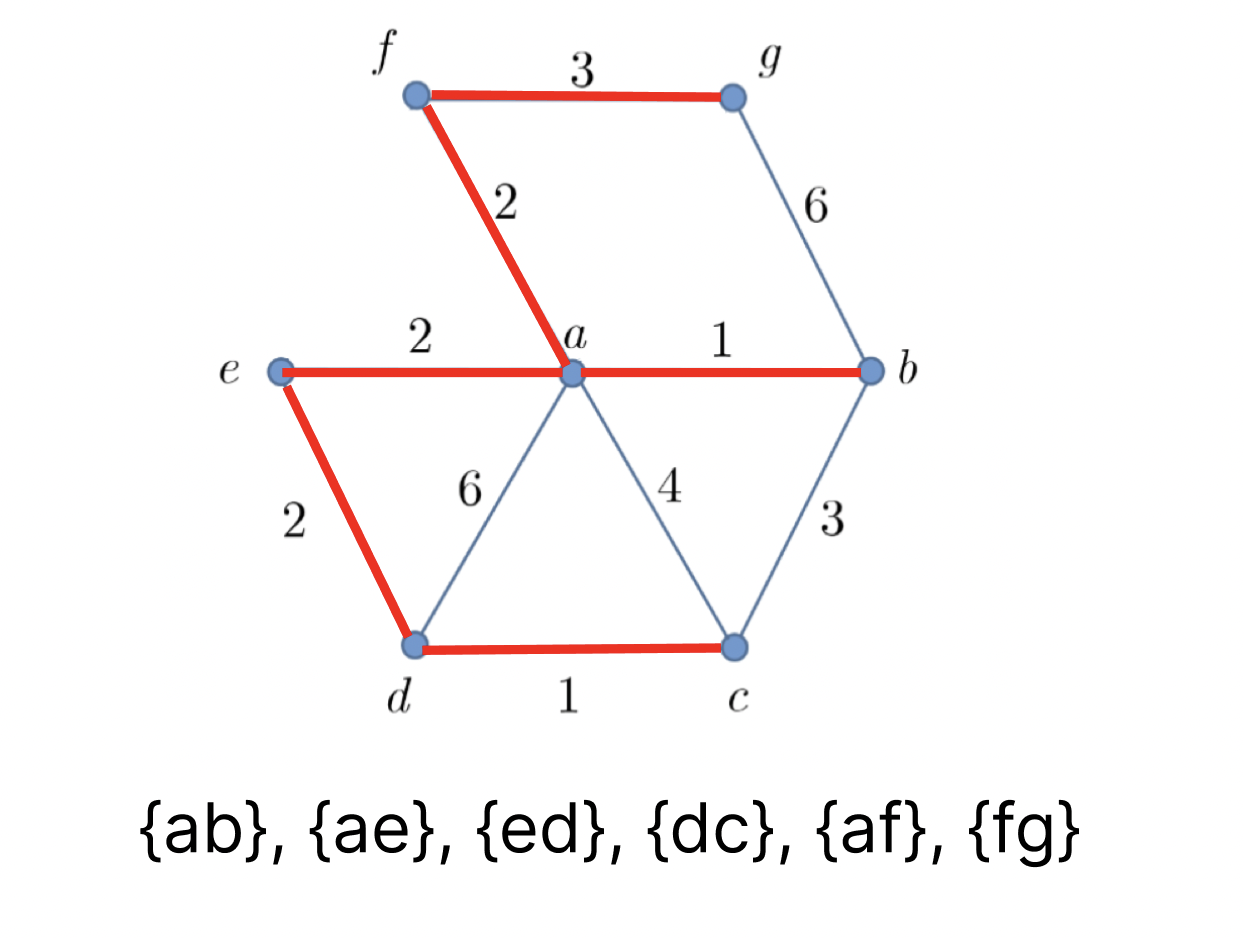
\includegraphics[scale=0.35]{prims.png}
%         \caption{}
%     \end{minipage}    
%     \qquad
%     \begin{minipage}{.4\textwidth}
%         \centering
%         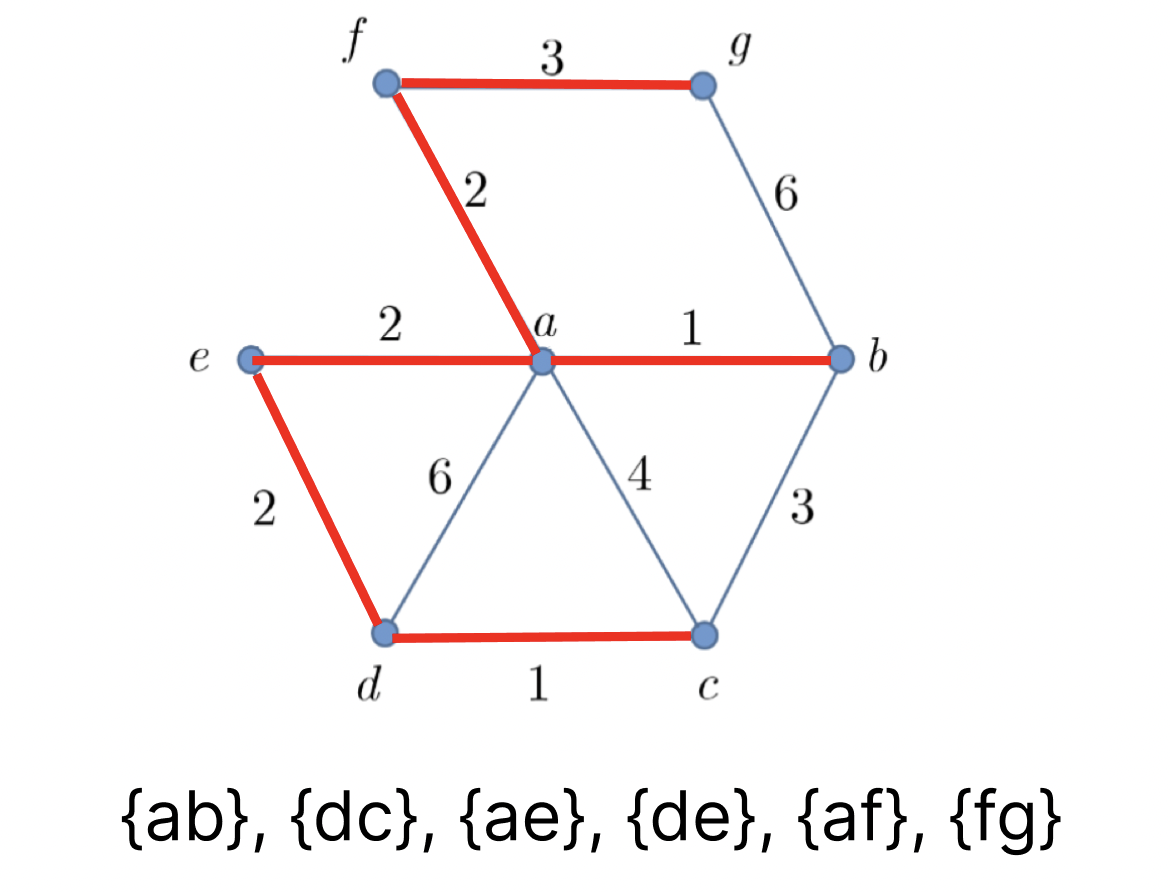
\includegraphics[scale=0.35]{kruskal.png}
%         \caption{}
%     \end{minipage}        
% \end{figure} 

\newtheorem{thm}{Theorem}
\newtheorem{proposition}[thm]{Proposition}
\newtheorem{cor}[thm]{Corollary}

% title information
\title{Math 110 Practice}
\author{Neo Lee}
\date{}

\setstretch{1.15}
% main content
\begin{document} 

% placing title information; comment out if using fancyhdr
\maketitle 

\section*{Midterm}
\begin{proposition}
    Let $V=\mathcal{P}_2(\mathbb{R})$. Let $I$ denote the identity map on $V$, $D$ the 
    differentiation map, $D^2=D\circ D$ the second differentiation map, and $T$ the map 
    $f(x)\mapsto f(x-1)$. Then the list $(I, D, D^2, T)$ are linearly dependent in $\mathcal{L}(V)$.
\end{proposition}
\begin{proof}
    We can write $ax^2 + bx + c \in\mathbb{P}_2(\mathbb{R})$. We want to find non-trivial solution 
    to the equation for any arbitrary $a, b, c \in\mathbb{R}$.
    \begin{align*}
        \alpha I(ax^2+bx+c) + \beta D(ax^2+bx+c) + \gamma D^2(ax^2+bx+c) + \delta T(ax^2+bx+c) & = 0 \\
        \alpha(ax^2+bx+c) + \beta(2ax+b) + \gamma(2a) + \delta(a(x-1)^2+b(x-1)+c) & = 0 \\
        \alpha(ax^2+bx+c) + \beta(2ax+b) + \gamma(2a) + \delta(ax^2-2ax+bx+a-b+c) & = 0 \\
        a(\alpha x^2+2\beta x+2\gamma+\delta x^2-2\delta x+\delta) + b(\alpha x +\beta +\delta x-\delta) 
        + c(\alpha + \delta) & = 0 \\
        a\left((\alpha+\delta)x^2+(2\beta-2\delta)x+2\gamma+\delta\right) + b\left((\alpha+\delta)x
        +\beta-\delta\right) + c(\alpha+\delta) & = 0.
    \end{align*}
    Since $a,b,c$ are free variables, we must have 
    \begin{align*}
        & \begin{cases}
            (\alpha+\delta)x^2+(2\beta-2\delta)x+2\gamma+\delta & = 0 \\
            (\alpha+\delta)x+\beta-\delta & = 0 \\
            \alpha + \delta & = 0
        \end{cases} \\
        \implies & \begin{cases}
            \alpha+\delta & = 0 \\
            2\beta-2\delta & = 0 \\
            2\gamma + \delta & = 0 \\
            \alpha + \delta & = 0 \\
            \beta - \delta & = 0 \\
            \alpha + \delta & = 0
        \end{cases} \qquad \because x^2, x, 1 \text{ are linearly independent}\\
        \implies & \begin{cases}
            \alpha+\delta & = 0 \\
            2\beta-2\delta & = 0 \\
            2\gamma + \delta & = 0.
        \end{cases} \\
        \implies & \begin{cases}
            \delta & = \delta \\
            \alpha & = -\delta \\
            \beta & = \delta \\
            \gamma & = -\frac{1}{2}\delta.
        \end{cases}
    \end{align*}
    Therefore, there exists infinitely non-trivial solutions to the equation, and the list is 
    linearly dependent.
\end{proof}

\begin{proposition}
    Let $V=\mathbb{R}^4$, let $W_1=\{(x_1,x_2,x_3,x_4):x_2+x_4=0, x_j\in\mathbb{R}
    \text{ for all }j\}$, and let $W_2=\{(x_1,x_2,x_3,x_4):x_1+x_2+x_3=0, x_j\in\mathbb{R}
    \text{ for all }j\}$. Then \begin{enumerate}[label=(\alph*)]
        \item $W_1$ and $W_2$ are subspaces of $V$;
        \item $\dim W_1\cap W_2 = 2$;
        \item $W_1 + W_2$ is not a direct sum and $\dim(W_1+W_2)$
    \end{enumerate}
\end{proposition}
\begin{proof}\indent
    \begin{enumerate}[label=(\alph*)]
        \item $W_1$ and $W_2$ obviously contain the zero vector by letting $x_1=x_2=x_3=x_4=0$.
        
        Both spaces are closed under addition. For $W_1$, let $u=(u_1,u_2,u_3,u_4), 
        v=(v_1,v_2,v_3,v_4)\in W_1$. Then $$u+v=(u_1+v_1, u_2+v_2, u_3+v_3, u_4+v_4),$$
        and $$(u+v)_2 + (u+v)_4 = (u_2+v_2) + (u_4+v_4) = (u_2+u_4) + (v_2+v_4)=0.$$ Similarly, for 
        $W_2$, let $u=(u_1,u_2,u_3,u_4), v=(v_1,v_2,v_3,v_4)\in W_2$. Then $$u+v=(u_1+v_1, u_2+v_2, 
        u_3+v_3, u_4+v_4),$$
        and $$(u+v)_1 + (u+v)_2 + (u+v)_3 = (u_1+v_1) + (u_2+v_2) + (u_3+v_3) = (u_1+u_2+u_3) + 
        (v_1+v_2+v_3)=0.$$

        Also, both spaces are closed under scalar multiplication. For $W_1$, let $u=(u_1,u_2,u_3,u_4)
        \in W_1$ and $\lambda\in\mathbb{R}$. Then $$\lambda u = (\lambda u_1, \lambda u_2, 
        \lambda u_3, \lambda u_4),$$ and $$(\lambda u)_2 + (\lambda u)_4 = \lambda u_2 + \lambda u_4
        = \lambda(u_2+u_4)=0.$$ Similarly, for $W_2$, let $u=(u_1,u_2,u_3,u_4)\in W_2$ and
        $\lambda\in\mathbb{R}$. Then $$\lambda u = (\lambda u_1, \lambda u_2, \lambda u_3,
        \lambda u_4),$$ and $$(\lambda u)_1 + (\lambda u)_2 + (\lambda u)_3 = \lambda u_1 +
        \lambda u_2 + \lambda u_3 = \lambda(u_1+u_2+u_3)=0.$$

        \item 
        We can write $W_1 = \{(x_1, -x_4, x_3, x_4:x_j\in\mathbb{R})\} = 
        \mathrm{span}\left\{\begin{bmatrix}
            1 \\ 0 \\ 0 \\ 0
        \end{bmatrix},\begin{bmatrix}
            0 \\ -1 \\ 0 \\ 1
        \end{bmatrix}, \begin{bmatrix}
            0 \\ 0 \\ 1 \\ 0
        \end{bmatrix}
        \right\}$. Similarly, we can write $W_2 = \{(x_1, -x_1-x_3, x_3, x_4:x_j\in\mathbb{R})\} =
        \mathrm{span}\left\{\begin{bmatrix}
            1 \\ -1 \\ 0 \\ 0
        \end{bmatrix},\begin{bmatrix}
            0 \\ -1 \\ 1 \\ 0
        \end{bmatrix}, \begin{bmatrix}
            0 \\ 0 \\ 0 \\ 1
        \end{bmatrix}
        \right\}$. Putting all their basis vectors together and reducing the matrix, we have 
        4 linearly independent vectors, and therefore $\dim (W_1+W_2)=4$. Hence, 
        $$\dim W_1 \cap W_2 = \dim W_1 + \dim W_2 - \dim (W_1+W_2) = 3 + 3 - 4 = 2.$$

        \emph{Alternatively,} we can denote the intersection $W_1\cap W_2=\{(x_1,x_2,x_3,x_4):
        x_2+x_4=0, x_1+x_2+x_3=0\}$, then $$W_1\cap W_2 = 
        \begin{bmatrix}
            x_1 \\ x_2 \\ -x_1-x_2 \\ -x_2
        \end{bmatrix} = \begin{bmatrix}
            x_1 \\ 0 \\ -x_1 \\ 0
        \end{bmatrix} + \begin{bmatrix}
            0 \\ x_2 \\ -x_2 \\ -x_2
        \end{bmatrix} = \mathrm{span}\left\{\begin{bmatrix}
            1 \\ 0 \\ -1 \\ 0
        \end{bmatrix}, \begin{bmatrix}
            0 \\ 1 \\ -1 \\ -1
        \end{bmatrix}\right\}.$$ Therefore, $\dim W_1\cap W_2 = 2$.
        \item 
        $\dim W_1\cap W_2 = 2\implies W_1\cap W_2\neq \{0\}\implies W_1\not\oplus W_2$. 
        $\dim (W_1+W_2) = \dim W_1 + \dim W_2 - \dim W_1\cap W_2 = 4$.
    \end{enumerate}

\end{proof}
\begin{proposition}
    Let $V$ be the vector space of all trigonometric polynomials (in $x$) with real 
    coefficients of degree at most 2, i.e. $V:=\mathrm{span}\{1,\sin x, \cos x, \sin(2x), 
    \cos(2x)\}$. The list $(1,\sin x, \cos x, \sin (2x), \cos(2x))$ is a basis of $V$. 
    Consider the linear operator 
    $$T\in\mathcal{L}(V):(Tf)(x)=f''(x)+f(x).$$
    \begin{enumerate}[label=(\alph*)]
        \item Find the matrix representation of $T$ in this basis used for the domain and the 
        codomain.
        
        \item Show $\dim \mathrm{null}T=2, \dim\mathrm{range}T=3$.
    \end{enumerate}
\end{proposition}
\begin{proof}\indent
    \begin{enumerate}[label=(\alph*)]
        \item 
        \begin{align*}
            (T1)(x) & = 0 + 1 = 1 \\
            (T\sin x)(x) & = -\sin x + \sin x = 0 \\
            (T\cos x)(x) & = -\cos x + \cos x = 0 \\
            (T\sin(2x))(x) & = -4\sin(2x) + \sin(2x) = -3\sin(2x) \\
            (T\cos(2x))(x) & = -4\cos(2x) + \cos(2x) = -3\cos(2x).
        \end{align*}
        We have determined the image of the basis vectors. Now we can write the matrix
        representation of $T$ in this basis used for the domain and the codomain. 
        $$\mathcal{M}(T) = \begin{bmatrix}
            1 & 0 & 0 & 0 & 0 \\
            0 & 0 & 0 & 0 & 0 \\
            0 & 0 & 0 & 0 & 0 \\
            0 & 0 & 0 & -3 & 0 \\
            0 & 0 & 0 & 0 & -3
        \end{bmatrix}.$$

        \item 
        Notice the image of $T$ is determined by $\mathcal{M}(T)\vec{v}$ for $\vec{v}\in 
        V$ represented as a column vector in terms of the basis. Therefore, range$T$ is 
        the same as the column space of $\mathcal{M}(T)$. We can see obviously that the 
        column space has dimension 3 since first column has non-zero entry at different 
        coordinates. Therefore, $$\dim\mathrm{range}T=3$$ and 
        $$\dim\mathrm{null}T=\dim V-\dim\mathrm{range}T=5-3=2.$$
    \end{enumerate}
\end{proof}

\begin{proposition}
    Consider the linear map $T:\mathcal{P}_2(\mathbb{R})\to\mathcal{P}_4(\mathbb{R}):f(x)\mapsto
    f(x^2)$ and the linear functional $\varphi:\mathcal{P}_4(\mathbb{R})\to\mathbb{R}:
    f(x)\mapsto f''(0)$. Then 
    \begin{enumerate}[label=(\alph*)]
        \item $T'(\varphi):\mathcal{P}_2(\mathbb{R})\to\mathbb{R}$;
        \item $T'(\varphi):ax^2+bx+c\mapsto 2b$;
        \item $\dim \mathrm{null}T' = 2$ and $T'$ is not an isomorphism.
    \end{enumerate}
\end{proposition}
\begin{proof}\indent
    \begin{enumerate}[label=(\alph*)]
        \item $T'(\varphi) = \varphi(T):\mathcal{P}_2(\mathbb{R})\to\mathcal{P}_4(\mathbb{R})
        \to \mathbb{R} = \mathcal{P}_2(\mathbb{R})\to \mathbb{R}$.
    
        \item 
        Consider arbitrary $ax^2+bx+c\in\mathbb{P}_2(\mathbb{R})$, 
        \begin{align*}
            T'(\varphi)(ax^2+bx+c) = \varphi(T)(ax^2+bx+c) & = \varphi(ax^4+bx^2+c) \\
            & = (ax^4+bx^2+c)''(0) \\
            & = (12ax^2+2b)_{x=0} \\
            & = 2b.
        \end{align*}

        \item 
        Notice $\mathrm{null}T' = (\mathrm{range}T)^0$, the annihilator of 
        range$T\in\mathcal{P}_4(\mathbb{R})$, and range$T=\mathrm{span}\{1,x^2,x^4\}$. 
        Then 
        \begin{align*}
            \dim \mathrm{null}T' & = \dim (\mathrm{range}T)^0 \\
            & = \dim \mathcal{P}_4(\mathbb{R})-\dim \mathrm{range}T \\
            & = 5 - 3 \\
            & = 2.
        \end{align*}

        Since $\dim \mathrm{null}T' = 2\neq 0$, $T'$ is not injective and therefore not an 
        isomorphism.
    \end{enumerate}
\end{proof}

\end{document}
